\documentclass[usegeometry=true]{scrartcl}
\usepackage[ngerman]{babel}
\usepackage[T1]{fontenc}
\usepackage{lmodern}
\usepackage[utf8]{inputenc}
\usepackage{hyperref}
\usepackage{amssymb}
% Dimensionen bitte nicht ändern. 
\usepackage[left=2cm, right=2cm, top=2cm, bottom=2cm, bindingoffset=1cm, includeheadfoot]{geometry}
%Zeilenabstand bitte nicht ändern
\usepackage[onehalfspacing]{setspace}

%--- Wrap text around figures
\usepackage{wrapfig}

% --- Abkürzungsverzeichnis ---
\usepackage[nohyperlinks, 
withpage, 
smaller,
footnote
]{acronym}



% --- Grafiken ---
\usepackage{graphicx}
\usepackage{subfig}



\usepackage[backend=biber,style=numeric,]{biblatex}\addbibresource{Visualisierung.bib}

\begin{document}
\pagenumbering{Roman}

\begin{titlepage}
	\begin{center}
		\large{\textsc{Martin-Luther-Universität Halle-Wittenberg}}\\
				

		\setstretch{1.5}
		Projektbericht zum Modul Information Retrieval und Visualisierung Sommersemester 2021
	\end{center}

	\begin{center}
		\Large
		\textbf{Visualisierung von Daten des Videospiels Fifa 21}
	\end{center}

	\vskip 1cm

	\vskip 0.75cm

	\begin{center}
		\begin{tabular}{lll}
			Eingereicht bei:& & Dr. Alexander Hinneburg\\
			Eingereicht von:  & & Johannes Lange \\
			Git-Repository: & & \url{https://github.com/JohannesLange/Visualisierung_FIFA19}\\
			%& & 06112 Halle (Saale)\\
			& & \\
			Eingereicht am: & & \today
		\end{tabular}
	\end{center}

\end{titlepage}



% ----------------------------------------------------------------------------

\newpage
%----------------------------------------------------------------------------
% Inhaltsverzeichnis:
\tableofcontents
\newpage

% Abbildungsverzeichnis
\clearpage
\addcontentsline{toc}{section}{Abbildungsverzeichnis}
\listoffigures

% Abkürzungsverzeichnis:
\section*{Abkürzungsverzeichnis}\label{AV}
	\addcontentsline{toc}{section}{Abkürzungsverzeichnis}
	\begin{acronym}
	\acro{CB}[CB]{Centerback}
	\acro{FUT}[FUT]{Fifa Ultimate Team}
	\acro{RB}[RB]{Rightback}
	\end{acronym}
\newpage
% ----------------------------------------------------------------------------
% Gliederung und Text:
\pagenumbering{arabic}
\section{Einleitung}

% -Zu Parallel Koordinaten on Hover inklusive der verglichenen Werte hinzufügen
% -Aggregationsfunktion möglicherweise entfernen, überprüfen ob der Code deutlich schneller läuft
% -Torhüter herausfiltern, da diese keine Werte haben
% -Filter Funktion in parallelen Koordinaten und Scatterplot erweitern
%Tipps zu Latex und Koma-Script für Hausarbeiten sind im \href{http://mirrors.ctan.org/info/latex-refsheet/LaTeX_RefSheet.pdf}{LaTeX Reference Sheet for a thesis with KOMA-Script} von Marion Lammarsch und Elke Schubert zusammengefasst. 
%Der Bericht fällt in die Kategorie von InfoVis-Paper, die Tamara Munzner Design Study nennt \cite{Munzner2008}: In der Einleitung sollen sie zuerst das Zielproblem beschrieben. Daraus sollen sie Fragestellungen motivieren, die mittels Techniken der Informationsvisualisierung beantwortet werden können. 

%\textbf{Tamara Munzner angucken}\\
%\textbf{Zielprobelm formulieren und daraus Fragestellung schreiben -> Wie können diese mittels Visualisierung beantwortet werden}


Die Visualisierung von Daten nimmt mit Hinblick auf Big Data und damit immer unübersichtlicheren Datengrundlagen an Bedeutung zu. Um aus großen Mengen von Daten neue Informationen zu gewinnen reicht es oft nicht aus die Daten direkt zu analysieren. Durch die Anwendung der richtigen Visualisierungstechniken können neue Informationen gewonnen werden.\\
Besonders Fans von kompetetiven Videospielen versuchen oft jeden möglichen Vorteil zu nutzen um gewinnen zu können.
Das Spiel FIFA 21, dessen Daten in dieser Arbeit visualsiert werden, bildet dabei keine Ausnahme.
Früher sind dazu häufig Guides verwendet worden in denen hunderte Seiten Tipps und Tricks abgedruckt worden sind. Diese Guides bieten jedoch keine Interaktion und sind oft aus der subjektiven Sicht eines einzelnen Autors verfasst. 
Moderne Visualisierungstechniken erlauben es deutlich mehr Informationen zu extrahieren und für die Spieler interaktiv nutzbar zu machen.
Aus diesem Grund sollen in dieser Designstudie drei Visualisierungstechniken vorgestellt werden die sich dafür eigenen den gegebenen Datensatz zu visualisieren um neue Erkenntnisse zu erhalten.
Dieser Datensatz ist äußerst umfangreich - zu über 16000 Sportlern sind jeweils 107 Variablen festgehalten. Diese reichen von \textit{Name} über \textit{Verein} bis hin zu \textit{Schusskraft} eines Spielers.
Zwar sind diese Daten dem Videospiel FIFA 21 entnommen, Daten wie \textit{Name, Alter, Verein, Nationalität, Größe} und \textit{Gewicht} beruhen aber auf echten Daten der Spieler. Weiterhin versucht der Hersteller des Spiels auch die restlichen Daten so nah an der Realität zu verankern wie möglich.
Dadurch besteht die Hoffnung mittels Visualisierungstechniken noch weitgreifendere Erkenntnisse aus dem gegebenen Datensatz ziehen zu können, als solche die lediglich Fans des Spiels dienen.\\
Mögliche Anforderungen an die Visualisierungen von Spielern des Spiels könnten dabei bspw. die Folgenden sein. Welcher Fussballer verbessert das Team kostet aber vergleichsweise wenig: \textit{Welche Spieler hat das höchste Overall bei geringstem Wage?}\\
Eine Weitere Frage könnte sich beim Bau eines Teams bestehend aus Bundesliga Vereinen ergeben, wenn ein Spieler einer bestimmten Position benötigt wird: \textit{Welche Linksverteidiger spielen in der Bundesliga?}\\
Außerdem könnten sich Fragen nach den besten Spielern bezüglich individueller Kriterien ergeben: \textit{Welcher Stürmer ist schnell, Schussstark, kann gut dribbeln und ist groß?}\\
Ob Fragen von anderen Anforderungsgruppen, wie bspw. Sportwissenschaftlern beantwortet werden können: \textit{Wann erreichen Fussballer ihren Peak? Sind größere Fussballer besser, schneller, etc.?} ist dabei nicht klar. Da alle Daten, die nicht konkret der Realität entnommen werden können, von Mitarbeitern des Herstellers festgelegt worden sind können diese nicht ohne weitere Analyse genutzt werden. Trotzdem lohnt es sich dies zu überprüfen und mit anderen wissenschaftlichen Arbeiten abzugleichen.

\newpage


\subsection{Anwendungshintergrund}
%Sie müssen genug Hintergrund bereitstellen, so dass die Lesenden sich ein Urteil bilden können, ob ihre Lösung funktioniert. Sie sollen die Lesenden jedoch nicht mit Anwendungsdetails so überschütten, dass der Fokus auf die Fragen zur Informationsvisualisierung untergehen. 
%\textbf{Was sind die Daten, sind die Visualisierungslösungen angebracht, möglicherweise auf einzelne Variablen eingehen}\cite{Munzner2008}

Im folgenden werden die drei verwendeten Visualisierungstechniken kurz vorgstellt und erklärt.
Bei der ersten Visualisierungstechnik handelt es sich um einen Scatterplot.\cite{noauthor_complete_nodate} Mit diesem lassen sich Zusammenhänge zwischen zwei verschiedenen, numerischen Attributen der Fussballer genauer untersuchen. So können Trends in Daten aufgezeigt werden, z.B. ob sich das Alter von Fussballern auf deren Bewertung im Spiel auswirkt.
Weiterhin können so Spieler gefunden werden deren Werte von den gefundenen Trends abweichen.\\
Die zweite Visualisierungstechnik ist die der Parallelen Koordinaten.\cite{few_multivariate_2006} Diese eignet sich aufgrund ihrer Beschaffenheit dazu mehrdimensionale Daten auf übergreifende Trends zu untersuchen. Trotzdem können sie auch genutzt werden um spezifische Fussballer konkret zu untersuchen und deren Werte im Vergleich zu den beschriebenen Trends zu betrachten. Bspw. kann der Frage nach der Eignung eines Fussballers zum Einsatz auf einer spezifischen Position nachgegangen werden.
Diese Darstellungsform ermöglicht den Vergleich vier verschiedener Attribute der Fussballer. Dabei ist allerdings zu beachten, dass Zusammenhänge innerhalb der Daten nur im Vergleich mit anderen Daten zu erkennen sind. Enthält der Datensatz bspw. nur einen Spieler zeigen die parallelen Koordinaten nur eine gerade Linie an. Weiterhin lassen sich lediglich Zusammenhänge zwischen benachbarten Attributen erkennen. Dies kann bei ungeschulten Anwendern schnell zu Fehlinterpretationen führen.\\
Bei der dritten Visualisierungstechnik handelt es sich um die explizite Baumdarstellung. Durch sie kann ein Überblick über hierarchische Strukturen ermöglicht werden. In diesem Fall ist dies die Fussballliga als oberstes Element, darauf folgen die Vereine der Liga und zum Schluss die Fussballer der Vereine. Von den drei Techniken ist diese aufgrund ihrer Bekanntheit vermutlich am einfachsten zu verstehen.


%Da diese Darstellungsform sehr schnell unübersichtlich werden kann sind die Daten nach Ligen gefiltert. Weiterhin können diese Daten noch nach Positionen gefiltert werden. So kann ein Spieler des FUT Modus, der für sein Team einen Linksverteidiger der Bundesliga benötigt nach dieser Liga und Position filtern.

%Die Frage, welche sich bei diesen Daten stellt ist, welchen Nutzen sie außerhalb eines Videospiels haben. Deswegen ist mein Ansatz zu vergleichen wie genau diese Daten die Wirklichkeit widerspiegeln. Ein Beispiel dafür könnte sein ob sich das Rating eines Spielers mit der körperlichen Entwicklung eines Spielers bewegt. Sollte dies zutreffen  müssten Spieler im Alter ihres physischen Peaks das höchste Rating haben. 
\subsection{Zielgruppen}
%Beschreiben sie die Personengruppe oder Personengruppen, die das von ihnen benannte Anwendungsproblem lösen möchte. Auf welches Vorwissen können sie in dieser Gruppen von Anwenderinnen aufbauen? Welche Informations"-bedürf"-nisse werden durch die Visualisierungen adressiert?
Da es sich bei den Daten um die eines Videospiels handelt ist davon auszugehen, dass eine der Zielgruppen Spieler des Videospiels sind. Diese sind weiterhin in die des Spielmodus \textit{Karriere} und die des Spielmodus \textit{Fifa Ultimate Team  FUT} zu unterteilen.\\
Spieler des FUT Modus sammeln die Fussballer wie in einer Art Sammelkarten Spiel. Mit den Karten der Fussballer (Siehe Abbildung \ref{Ronaldo}) kann dann Online gegen andere Spieler angetreten werden.
Dabei sind sechs verschiedene Werte der Fussballer von Relevanz (Siehe Werte in Abbildung \ref{Ronaldo}). Da dieser Modus sehr kompetetiv ist kann ein Fussballer bereits durch einen einzigen schlechten Wert für Spieler unbrauchbar werden.
Dadurch, dass \textit{FUT} zu den Onlinespielen gehört in denen viele Spieler sich durch \textit{Min-Maxing}\cite{noauthor_min-maxing_2014} einen Vorteil verschaffen wollen ist bei den Anwendern von einem hohen Vorwissen bezüglich der Daten auszugehen. Mit Blick auf die Visualisierungetechniken nicht davon auszugehen, dass die Funktionsweise der Parallelen Koordinaten bekannt ist. Da diese Gruppe genug Interesse aufweist um bereit zu sein Zeit in das Verständnis einer Visualisierungstechnik zu investieren, bietet sich diese Technik allerdings trotzdem an. Eine weitere für diese Gruppe relevante Visualisierungstechnik ist die explizite Baumdarstellung, durch diese ist es möglich zu untersuchen welche Spieler in welcher Liga und welchem Team spielen. Dadurch können Spieler dabei unterstützt werden ihr Team passend zusammenzustellen. Das Funktionsweise eines Baumdiagramms sollte dabei den meisten Spielern bereits bekannt sein.\\
Spieler des Karrieremodus spielen das Spiel als Manager eines Vereins. In diesem Spielmodus ist die Entwicklung von jungen Spielern wichtig. Vor allem der Vergleich von Variablen wie \textit{Wage, Age, Overall} oder \textit{Potential} ist dabei relevant. In diesem Fall bietet sich eine Darstellung per Scatterplot an. Mit dieser Technik lassen sich schnell die aussichtsreichsten Fussballer erkennen. Da der Karrieremodus nicht Online gespielt wird und die Schwierigkeit manuell festgelegt werden kann, ist davon auszugehen, dass das Vorwissen der Gruppe stark schwankt. Während einige Spieler bereits viel Wissen haben und deswegen sehr genaue Informationen benötigen um auf dem höchsten Schwierigkeitsgrad bestehen zu können, benötigen andere erst einmal Grundwissen bezüglich der Spieler. Aus diesem Grund bietet sich auch die Visualisierung mittels eines Baumdiagramms an. Durch diese kann sich ein grober Überblick über Spieler einer Liga gemacht und durch die Möglichkeit des Filterns nach Positionen können grob auch Spieler gescouted werden. Aufgrund des geringen Bedarfs an besonders spezifischen Informationen im Vergleich zum FUT Modus ist nicht mit genügend Ansporn zum Erlernen der Funktionsweise von parallelen Koordinaten zu rechnen. Die Funktionsweise eines Scatterplots sowie eines Baumdiagramms sollte aber den meisten Mitgliedern dieser Zielgruppe bereits bekannt sein.


\begin{wrapfigure}{l}{0.5\textwidth}
\centering
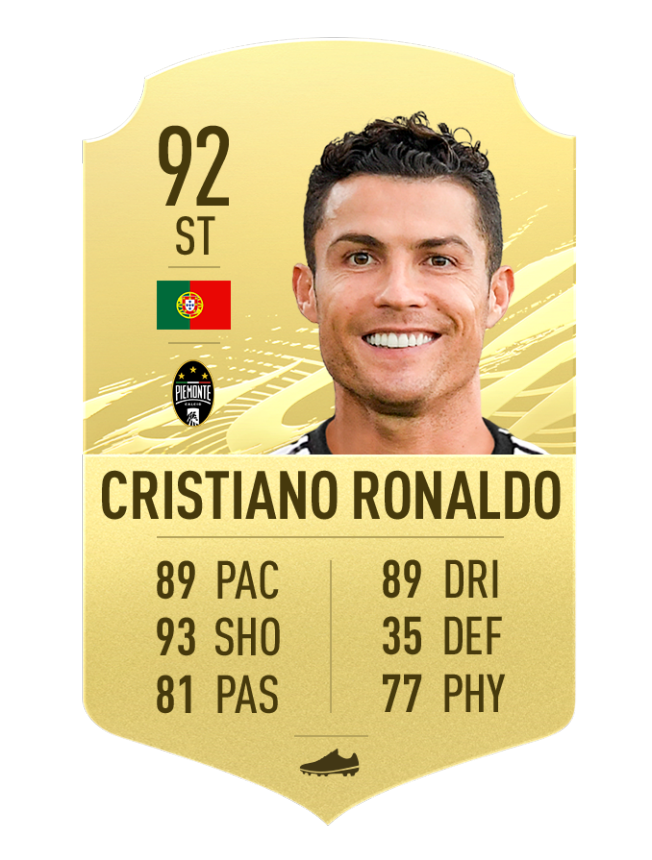
\includegraphics[scale=0.15]{grafiken/Ronaldo}
\caption{Darstellung einer FUT Karte inklusive relevanter Werte am Beispiel Cristiano Ronaldo\\ Quelle: https://www.ea.com/de-de/games/fifa/fifa-21/news/fifa-21-player-ratings-best-strikers-st-cf}
\label{Ronaldo}
\end{wrapfigure}

Bei der dritten Zielgruppe, den Sportwissenschaftlern ist von genügend Vorwissen bezüglich der Daten sowie aller Visualisierungstechniken auszugehen. Bei ihnen stellt sich allerdings noch immer die Frage, welchen Mehrwert ihnen die Visualisierungstechniken bieten können. Beim Baumdiagramm ist dabei von keinem Nutzen auszugehen. Scatterplot und parallele Koordinaten könnten, nach Analyse der Daten auf Realitätsnähe, dazu genutzt werden mögliche Fragestellungen zu beantworten. Weiterhin ist zu sagen, dass dieser Zielgruppe vermutlich nur Erkenntnisse über Trends innerhalb des Datensatzes behilflich sein werden, nicht aber Informationen über spezifische Fussballer.\\

\subsection{Überblick und Beiträge}
%In diesem Abschnitt geben sie einen kurzen Überblick über die Daten und verwendeten Visualisierungen. Dann benennen sie die Beiträge ihres Projekts. Diese Beiträge müssen sie in den hinteren Teilen des Berichts genauer ausführen und belegen.

Wie bereits beschrieben sind Guides zu Videospielen bisher meist in Papierform veröffentlicht worden und sind wenig interaktiv. Da das Informationsbedürfnis von Spielern gerade in den letzten Jahren stark zugenommen hat, bietet sich der Einsatz von Visualisierungstechniken auf Basis von Daten, welche das Spiel selbst liefert an. Dadurch ist es möglich den gesteigerten Informationsbedarf zu decken ohne direkt Programmierkenntnisse beim Spieler vorauszusetzen.
Für die Visualisierungstechnik Scatterplot ist sich vor allem aufgrund dessen Verbreitung und Simplizität entschieden worden. Da es sich bei den möglichen Zielgruppen zum Großteil nicht um wissenschaftler handelt bietet der Scatterplot eine verständliche Visualisierung an, die aber trotzdem einen deutlichen Mehrwert gegenüber den Daten in rein tabellarischer Form aufweist.
Das Baumdiagramm ist aufgrund der Möglichkeit hierarchische Daten darstellen zu können, ausgewählt worden. So kann übersichtlich gezeigt werden welche Spieler in welchen Vereinen und welche Vereine in welcher Liga spielen.
Im Gegensatz zu diesen beiden Visualisierungen sind die Parallelen Koordinaten unbekannter und von Laien nicht direkt zu verstehen. Trotzdem gehören sie zu den verständlichsten Techniken um multidimensionale Daten in einem zweidimensionalen Raum darzustellen. Durch sie wird vor allem der interaktive Vergleich von mehr als zwei Attributen ermöglicht. 
Wie genau die Visualisierungen umgesetzt worden sind und welchen Mehrwert jede einzelne Technik gegenüber anderen Visualisierungsformen bietet ist in Kapitel 3 diskutiert. Wie Anforderungen spezifischer Nutzer befriedigt werden ist in Kapitel 5 beschrieben.

\iffalse



Die erste verwendete Visualisierungstechnik ist der Scatterplot, dieser ist gut dazu geeignet zwei Variablen der Fussballer zu vergleichen. Bspw. könnte untersucht werden ob ein Fussballer entsprechend seines Könnens (Rating) verdient (Wage). Für Spieler des Karrieremodus können gerade solche Informationen relevant sein, da so Spieler gefunden werden können, die besser spielen als ihr Gehalt es vermuten lassen würde oder solche die zu teuer für ihr können sind.\\

Bei der zweiten verwendeten Visualisierungstechnik handelt es sich um Parallele Koordinaten. Diese, im Vergleich zum Scatterplot, etwas fortgeschrittene Technik eignet sich um mehr als zwei Werte miteinander zu vergleichen. Ihr Einsatz bietet sich daher an um Werte eines Fussballers in den Attributen: Schießen, Passen, Dribbling, Verteidigen, Geschwindigkeit oder Physis miteinander zu vergleichen und dies vorher nach der Position des Fussballers zu Filtern um zu untersuchen ob sich ein Spieler anhand seiner Attribute dafür eignet auf dieser Position zu spielen. (Bsp. ein Stürmer benötigt vor allem Geschwindigkeit, Schießen und Dribbling, ein Verteidiger hingegen Verteidigen, Physis und Geschwindigkeit).
Diese Technik könnte besonders für Spieler des FUT Modus relevant sein, da sich so die besten Spieler für den kompetetiven Online-Modus finden lassen.\\

Die dritte Visualisierungstechnik ist die Darstellung als Baumdiagramm. durch sie werden Spieler ihren Teams und diese ihren jeweiligen Ligen zugeordnet. Da es im FUT Modus ein Chemie System gibt indem ein Team nur gut zusammenspielen kann wenn Spieler einer Liga oder eines Teams entstammen kann ein Nutzer der Visualisierung mit Hilfe dieser ein Team aus einer spezifischen Liga zusammen bauen und nach jeder einzelnen Position filtern\cite{heib_fifa_2021}.



Als dritte und letzte Technik habe ich die Baumdarstellung ausgewählt um sichtbar zu machen welche Fussballliga Europas im Durchschnitt die besten Spieler hat. Deswegen ist dies für X interessant.\\
\fi
\section{Daten}
%Beschreiben Sie vorhandenen Daten. Gehen sie kritisch darauf ein, in wie weit sich die Daten für die Bearbeitung der Fragestellungen und dem Erreichen von Lösungen für die oben beschriebene Zielgruppen eignen. Haben sie die Daten sinnvoll mit weiteren Datenquellen ergänzt? Wenn ja, wie?

%\textbf{Beschreibung der gegebenen Daten, Sind sie zur Beantwortung der Fragestellungen geeignet? Welche zusätzlichen Daten wurden genutzt} 
Bei den Daten handelt es sich um einen Datensatz des Fussball Videospiels Fifa 21\footnote{\url{https://www.kaggle.com/ekrembayar/fifa-21-complete-player-dataset} besucht am 10.09.2021}. Dieser ist der Website Kaggle entnommen. Dieser enthält Daten zu über 16000 Fussballern des Videospiels FIFA 21. In diesen enthalten sind neben Variablen wie Name, Verein und Alter auch ein ungefähr nach der Qualität des Fussballers festgelegte Bewertung sowie spezifischere Informationen zu den fussballerischen Fähigkeiten (Schießen, Passen, Dribbling, Verteidigen, Geschwindigkeit, Physis, etc.) der Spieler.\\
Grundsätzlich eignen sich die Daten gut um die genannten Fragestellungen beantworten zu können. Allerdings enthält der Grunddatensatz einige Felder, die für die Visualisierung nicht nötig sind, aus diesem Grund ist der Datensatz in der Vorvorarbeitung verkleinert worden (Siehe \ref{Datenvorverarbeitung}). Weiterhin ist der Datensatz nicht nur im Sinne der Attribute pro Fussballer sehr groß, sondern auch bezüglich der Anzahl an Fussbalern. Das führt bei allen verwendeten Visualisierungen dazu, dass Unübersichtlich werden. Um dies zu verhindern ist entschieden worden zusätzliche Filterfunktionalitäten einzubauen. %Da Datenwerte wie Größe, Alter und Rating der Spieler diskret sind, ist entschieden worden die Opazität der Punkte zu verringern, so ist zu erkennen an welchen Stellen sich mehrere Spieler überlagern. Da ab einer bestimmten Anzahl an Spielern die maximale Opazität erreicht ist und eine geringere Opazität pro Punkt einzelne Punkte fast unsichtbar machen würde, wird im Scatterplot beim hovern über einem Punkt angezeigt wie viele Spieler die genau gleichen  X und Y Werte aufweisen.

\subsection{Technische Bereitstellung der Daten}
%Wie sind die Daten zugänglich? Welche Formate werden genutzt. Gibt es Besonderheiten beim Lesen der Formate?
Die Daten sind in einem öffentlichen Github Repository gehostet\footnote{\url{https://github.com/JohannesLange/Visualisierung_FIFA19/tree/master}}. Dort liegen die Daten der drei Visualisierungen jeweils als \textit{.csv} vor. Die verwendeten Variablen sowie die Anzahl an Fussballern wurden jeweils der Visualisierungstechnik entsprechend angepasst um den Datensatz so klein wie möglich zu halten und so die Geschwindigkeit der jeweiligen Anwendung zu optimieren.
Auch die Daten der Visualisierung als Baumdiagramm liegen als \textit{.csv} vor. Sie werden erst im Programm zu einer \textit{.json} encoded und anschließend wieder zu einem Baumdiagramm decoded. So liegen die Daten nicht starr als \textit{.json} vor. Dies erlaubt das vorfiltern der Daten innerhalb des Programms. Da der Datensatz keine Daten bezüglich der Fussballligen, in denen die Vereine spielen, enthält, sind diese manuell eingefügt worden.


\subsection{\label{Datenvorverarbeitung}Datenvorverarbeitung}
%Welche Datenvorverarbeitungsschritte sind notwendig? Beschreiben Sie die einzelnen Schritte und begründen sie sie, z.B. warum werden manche Daten weggelassen, über welche Mengen werden Durchschnitte berechnet, warum sind die so berechneten Werte aussagekräftiger als andere Werte. 

Der Datensatz besteht aus Daten von über 16000 einzelnen Fussballern. Jeder dieser hat 107 einzelne Variablen. Da diese nicht alle relevant für die Visualisierungen sind und ein kleinerer Datensatz die Visualisierung beschleunigt, sind nur die relevanten Variablen ausgewählt worden. Da sich die relevanten Variablen auch zwischen den verschiedenen Visualisierungstechniken unterscheiden, sind für jede Anwendung unterschiedliche Datensätze vorverarbeitet und gefiltert worden.

Die Vorverarbeitung der Daten ist in \textit{R} durchgeführt worden. Das verwendete Skript (\textit{RDataPreprocessing.r}) liegt im Github vor.
Im ersten Schritt der Vorverarbeitung sind \textit{NA} Werte aus dem Datensatz entfernt worden.
Außerdem ist der Wert \textit{Height} von Fuß und Inch in Zentimeter umgewandelt worden um so eine Schreibweise ohne nicht-numerische Zeichen zu erhalten (Bsp.: \textit{6''2} wird zu \textit{188}). Weiterhin ist beim Wert \textit{Weight} die Beschriftung \textit{lbs} entfernt worden um den Wert so als numerischen Wert für den csv-Decoder von elm erkennbar zu machen.
Gleiches ist für die Werte \textit{Wage} und \textit{Value} getan worden. Bei diesen Werten ist die Umwandlung allerdings komplexer, da die Zahlen mit \textit{M} für Millionen und \textit{K} für Tausend abgekürzt sind.
Diese Werte sind ''in Tausend'' im finalen Datensatz enthalten. Werte die im Datensatz mit einem \textit{M} versehen sind, werden mit 1000 multipliziert, Werte mit \textit{K} sind entsprechend unverändert geblieben und Werte ohne Buchstaben sind durch 1000 geteilt worden (Bsp.: \textit{1.1M} ist zu \textit{1100} geworden, \textit{90K} zu \textit{90} und \textit{900} zu \textit{0.9}).
Sind diese Werte angepasst, können die für Scatterplot und Parallele Koordinaten relevanten Werte in jeweils neuen \textit{Data.frames} gespeichert und als \textit{.csv} wieder exportiert werden.\\
Für die Darstellung des Baumdiagramms ist sich auf die vier größten europäischen Fussballligen (Premier League, Bundesliga, La Liga und Serie A) konzentriert worden. Da im Datensatz keine Informationen zur Liga vorliegen sind die relevanten Spieler über eine manuell erstellte Liste der Vereine dieser Ligen gefiltert worden.Aus diesem Grund enthält der Datensatz dieser Visualisierungstechnik nur Daten von Spielern, deren Verein Teil einer dieser vier Ligen ist.

Im Git Repository sind unter dem Ordner \textit{data} der ursprüngliche, unveränderte Datensatz (\textit{fifa21\_male2.csv}) sowie die vorverarbeiteten Datensätze (Scatterplot: spData.csv, Parallele Koordinaten: pkData.csv, Baumdiagramm: baumData.csv) zu finden.

\section{Visualisierungen}
Im folgenden Kapitel werden die drei Visualisierungen vorgestellt. Dabei wird sowohl auf die jeweiligen Einsatzmöglichkeiten der Techniken, als auch auf Anforderungen, die sich aus den Bedürnissen der Zielgruppen ergeben, eingegangen. Weiterhin werden im weiteren Verlauf die Visualisierungen vorgestellt und Interaktionsmöglichkeiten beschrieben.  

\iffalse

Der gegebene Datensatz wird auf drei verschiedene Arten visualisiert.
Die erste Visualisierung ist ein Scatterplot. Mit diesem können zwei verschiedene Attribute des Datensatzes vom Nutzer freigewählt werden und die Spieler anhand dieser miteinander verglichen werden.\\
Bei der zweiten Visualisierungsform handelt es sich um parallele Koordinaten, diese erlauben im Vergleich zum Scatterplot den Vergleich von mehr als zwei Attributen, sind aber vergleichsweise unübersichtlicher. Weiterhin müssen Nutzer deutlich bewanderter sein um sie interpretieren zu können, da Zusammenhänge nicht benachbarter Attribute kaum erkenntlich sind und vom Nutzer erwartet wird diese nach Rechts und Links zu verschieben.\\
Die dritte Visualisierung ist ein explizites Baumdiagramm. Mit diesem kann die Struktur der Fussballligen Europas dargestellt werden. Dabei können Nutzer die Liga auswählen und die Spieler nach ihren Positionen filtern.


 Da der Datensatz sehr groß ist können die Spieler nach Verein und Nationalität noch zusätzlich gefiltert werden. Da es trotz dessen noch häufig Überschneidungen der Daten gibt, bspw. bei Alter und Overall der Spieler existiert eine Funktion, die anzeigt wie viele Spieler genau diese Werte aufweisen. Weiterhin sind die angezeigten Punkte teilweise durchsichtig. Dadurch können Überschneidungen der Punkte auch durch deren Opazität erkannt werden.

\fi

\subsection{Analyse der Anwendungsaufgaben}
%Analysieren sie die konkreten Anwendungsaufgaben. Welche Visualisierungen helfen den Personen, die die Software verwenden, sinnvolle mentale Modelle aufzubauen. Sind diese mentalen Modelle für sie notwendig, um die Aufgaben lösen zu können?
Die Visualisierungen sollen Nutzer dabei unterstützen neue Erkenntnisse aus Daten zu ziehen die ihnen ohne die Visualisierung verborgen bleiben würden oder nur mit erheblichem Zeitaufwand zu erkennen wären.
Dabei bieten Scatterplot und Parallele Koordinaten die Möglichkeit größere Trends innerhalb der Daten zu erkennen: \textit{Korrelieren Alter und Bewertung eines Fussballers? Sind teurere Fussballer besser?}
Aber auch Detailanforderungen wie die Suche nach einem Innenverteidiger, der die Wünsche des Nutzers bestmöglich erfüllt:\textit{Welcher Innenverteidiger hat einen besonders hohen Passwert bei akzeptablen Bewertungen der anderen relevanten Attribute?}
Durch die eingebaute Funktion, dass ein Pfad eines Spielers \textit{on:hover} die Farbe ändert und die genauen Werte des Spielers angezeigt werden kann auch ein spezieller Spieler aus der gesamten Liste gefiltert werden. So kann untersucht werden ob dessen Eigenschaften von den generellen Trends abweicht.
Ähnliches bewirkt die Funktion der Farbänderung und Namensanzeige \textit{on:hover} über Punkten des Scatterplots.
Dazu sei zu erwähnen, dass diese Funktion auch bei der Analyse größerer Trends hilfreich sein kann. Da sich viele diskrete Werte des Datensatzes überschneiden ist die Opazität der Punkte zwar bereits verringert worden. Eine weitere Reduzierung würde einzelne Punkte fast unsichtbar machen. Trotzdem ist durch die Größe des Datensatzes die maximale Opazität an an einigen Stellen schnell erreicht. Aus diesem Grund wird \textit{on:hover} neben dem Namen des Spielers auch die Anzahl an Spielern, die von diesem überlagert werden angezeigt. 
Im Vergleich zu diesen Techniken befriedigt das explizite Baumdiagramm andere Anforderungen. Mit ihm lassen sich Hierarchien darstellen. In Kombination mit der implementierten Filterfunktion lassen sich so Fragen nach Spielern bestimmter Positionen in den Ligen beantworten.\\

Insgesamt ist zu beachten, dass die Zielgruppen mit den Visualisierungsformen Scatterplot und Baumdiagramm vermutlich bereits in Kontakt gekommen sind und diese deswegen bereits interpretieren können. Parallele Koordinaten hingegen sind eine vergleichsweise unbekannte Visualisierungstechnik. Aus diesem Grund bietet es sich an den Parallelen Koordinaten eine Erklärung der Funktionsweise beizulegen. Dadurch kann den Nutzern geholfen werden diese Technik verstehen und nutzen zu können.

\subsection{Anforderungen an die Visualisierungen}
%Leiten sie Anforderungen an das Design der Visualisierungen ab, die sich durch ihre Analyse des Zielproblems ergeben.
%\textbf{Wie muss die Visualisierung designed werden um das Zielproblem gut beantworten zu können?}
Wie bereits im vorherigen Abschnitt beschrieben worden ist adressieren die Visualisierungen spezifische Ziele. Um diese Zielforderungen beantworten zu können, müssen sie auch deren Anforderungen erfüllen. In diesem Abschnitt wird aus diesem Grund die Designentscheidungen, welche sich aus den Anforderungen ergeben, erklärt.\\
Da es sich bei den Zielgruppen nicht um Programmierer handelt ist eine Anforderung an alle Visualisierungen eine verständliche Darstellung. Dazu gehört die verständliche Beschriftung der Achsen sowie passende farbliche Kodierung einiger Elemente. Ein weiterer Teil dieser Anforderung ist Übersichtlichkeit zu waren. Im Fall großer Datenmengen können Visualisierungen schnell unübersichtlich werden und so ihren Nutzen einbüßen. Aus diesem Grund sind in alle drei Visualisierungen verschiedene Filterfunktionen implementiert worden. Dies befriedigt eine weiteres Ziel: nur bestimmte Teilgruppen mit einander vergleichen zu können.\\
Eine weitere Designentscheidung ergibt sich aus dem Ziel spezifische Fussballer untersuchen zu können. Aus diesem Grund ist sowohl im Scatterplot als auch im Fall der Parallelen Koordinaten eine \textit{on:hover} Funktion implementiert worden, die den gewählten Punkt oder Pfad hervorhebt und Name sowie Informationen zu dem jeweiligen Fussballer anzeigt.
Um den Nutzern einen Mehrwert gegenüber analogen Visualisierungen zu bieten und den Bedarf selbstgewählter Vergleiche von Daten zu decken, ist in die Visualisierung des Scatterplots und der Parallelen Koordinaten die Möglichkeit eingebaut worden die zu vergleichenden Attribute selbst zu wählen.\\
Da Daten in Baumdiagrammen bei einer großen Menge an Kindern schnell unübersichtlich werden können ist im Baumdiagramm eine Filterfunktion nach Ligen und Positionen der Spieler implementiert worden. So kann sich fast ohne Scrollen ein Überblick über alle Spieler einer Position verschaft werden.\\


\subsection{Präsentation der Visualisierungen}

Im folgenden Kapitel werden die drei Visualisierungsformen vorgestellt. Weiterhin wird auf Funktionalität und Interaktionsmöglichkeiten genauer eingegangen.
%Präsentieren sie die visuelle Abbildungen und Kodierungen der Daten und Interaktionsmöglichkeiten. 
%Sie müssen  begründen, warum und wiegut ihre Designentscheidungen die erstellten Anforderungen erfüllen. 
%Weiterhin müssen sie begründen, warum die gewählte visuelle Kodierung der Daten für das zulösenden Problem passend ist. 
%Typische Argumente würden hier auf Wahrnehmungsprinzipien und Theorie über Informationsvisualisierung verweisen. 
%Die besten Begründungen diskutieren explizit die konkrete Auswahl der Visualisierungen im Kontext von mehreren verschiedenen Alternativen. Diskutieren sie die Expressivität und die Effektivität der einzelnen Visualisierungen. 

%Die eben beschriebenen Präsentationen und Begründungen sollen für jede der drei folgenden Visualisierungen durchgeführt werden. 

%\textbf{Visualisierungstechniken vorstellen, Interaktivität zeigen, Designentscheidungen begründen(Erfüllen diese die Anforderungen?), Diskutieren wieso nicht andere Techniken verwendet wurden(Expressivität und Effektivität).}
\subsubsection{Visualisierung Eins}
Bei der ersten Visualisierung handelt es sich um einen Scatterplot.
Mit diesem können zwei Attribute der Fussballer mit einander verglichen werden. Welche diese sind kann vom Anwender per Knopfdruck festgelegt werden. Im Scatterplot wird jeder Spieler als ein Punkt dargestellt. Da im Datensatz viele diskrete Werte existieren und deswegen viele Überlagerungen existieren, wurde die Opazität der einzelnen Punkte verringert. Dadurch ist es weiterhin möglich zu erkennen an welchen Stellen sich Daten fokussieren. Da die Opazität aber nicht unendlich verringert werden kann ist zusätzlich eine Funktion eingebaut, die beim \textit{hovern} mit der Maus über einem Punkt anzeigt wie viele andere Fussballer von diesem überlagert werden. Da diese Funktion die Laufzeit der Visualisierung deutlich erhöht ist unter dem Namen \textit{ScatterplotFast.elm} eine Version des Codes ohne diese Funktion enthalten.
Die X und Y Achse sind immer mit dem, vom Nutzer ausgewählten, Attribut beschriftet und skalieren bei Wechsel der Attribute automatisch mit.
Abschließend sei zu erwähnen, dass eine Filterfunktion für Vereine und Nationalitäten der Spieler implementiert worden ist. Dadurch ist es den Anwendern möglich die Aufmerksamkeit auf spezifische Teilgruppen zu richten und mögliche lokale Trends in den Daten zu erkennen.
Betrachtet man den Scatterplot im Vergleich zu anderen zweidimensionalen Visualisierungstechniken wie beispielsweise dem Balkendiagramm zeigt sich ein großer Vorteil des Scatterplots. Obwohl übergreifende Trends in den Daten zu erkennen sind lassen sich die Einzelobservationen noch voneinander differenzieren. Dieser Fakt ist in einigen der beschrieben Anwendungsfälle definitiv relevant.


\subsubsection{Visualisierung Zwei}
Bei der zweiten Visualisierung handelt es sich um die der Parallelen Koordinaten. 
Wie bereits beschrieben ist diese Visualisierungsform dafür geeignet höherdimensionale Daten in einem zweidimensionalen Raum darzustellen. Zwar benötigt diese Darstellungsform mehr als einzelne Datensätze um interpretierbar zu sein, trotzdem muss ein einzelner Datensatz erkennbar bleiben. Aus diesem Grund sind zum einen Filterfunktionen für die Attribute: Verein, Nationalität und Position eingebaut worden, zum anderen ist eine \textit{on:hover} Funktion implementiert worden, die den Pfad des ausgewählten Fussballers einfärbt, verbreitert und dessen Namen und Werte oberhalb der Darstellung anzeigt.
Da es für die Parallelen Koordinaten relevant ist ob Attribute benachbart sind oder nicht, ist genauso wie bei der Scatterplot Darstellung die Option implementiert worden die Werte der parallelen Achsen vom Nutzer selbst per Knopfdruck festlegen zu lassen.
Eine ähnliche Visualisierungsform zur zweidimensionalen Darstellung mehrdimensionaler Daten ist das Sterndiagramm. Zwar bietet dieses Vorteile wie beispielsweise den Fakt, dass kein Attribut am Ende allein ohne Nachbarn steht. Außerdem haben einzelne Observationen Aussagekraft ohne einen Vergleich mit anderen zu benötigen. Trotzdem ist die Verwendung der Parallelen Koordinaten bei den gegebenen Anforderungen die beste Wahl. Bei einem Datensatz mit der Größe des hier gegebenen wären die Daten im Sterndiagramm nicht zu erkennen. Generell ist diese Darstellungsform eher geeignet wenige Daten zu vergleichen und nicht große Datenmengen auf Trends zu untersuchen. 


\subsubsection{Visualisierung Drei}

Bei der dritten Visualisierung handelt es sich um die explizite Baumdarstellung. Diese Darstellungsform ist besonders dazu geeignet Hierarchien zu visualisieren. 
Die Hierarchie hat in diesem Fall drei Ebenen: Die Fussballliga, die Vereine und die Spieler.
Die Visualisierung hätte um Länder und Kontinente erweitert werden können. Dies ist allerdings nicht getan worden, da dadurch den Zielgruppen kein Mehrwert entstanden wäre.
Explizite Bäume sind eine Visualisierungstechnik die schnell in die breite wachsen und unübersichtlich werden können. Deswegen ist neben der Funktion einzelne Ligen auswählen zu können noch eine Filterfunktion nach Positionen implementiert worden. So wird die Darstellung entweder aller Spieler einer Liga oder aller Spieler einer bestimmten Position einer Liga ermöglicht. Ist das Visualisierungsziel das Darstellen von Hierarchien so gibt es verschiedene Techniken zur Auswahl. Diese reichen von Sunburstdiagrammen über implizite Baumdiagramme bis hin zu den Zur Zeit sehr beliebten Sankeydiagrammen. Trotzdem ist das explizite Baumdiagramm noch immer die leichtverständlichste und übersichtlichste Visualisierung hierarchischer Daten. Zwar wird ein Baumdiagramm bei einer großen Menge an Kinddaten schnell sehr breit, trotzdem sind die Daten zu erkennen. Sunburstdiagramme, Sankeydiagramme und implizite Baumdiagramme bieten zwar alle den Vorteil, dass die Größe ihrer Elemente zusätzliche Informationen übermitteln. Haben kleine Elternelemente allerdings viele Kinder sind diese oft kaum noch zu erkennen. Dieser Fall kann bei expliziten Baumdiagrammen nicht eintreten. Da in den Anforderungen lediglich die hierarchische Darstellung, nicht aber bestimmte Mengen relevant sind, ist die explizite Baumdarstellung gewählt worden.

\subsection{Interaktion}
%Erklären sie die möglichen Interaktionen mit den einzelnen Visualisierungen und die möglichen Verknüpfungen zwischen ihnen. Begründen Sie warum die konkreten Interaktionen umgesetzt wurden und welche Zwecke für die Anwenderinnen mit ihnen unterstützt werden. Begründen sie ebenfalls warum sie andere Interaktionsmöglichkeiten nicht umgesetzt haben. 

%\textbf{Interaktionen in den Visualisierungen(möglicherweise Interaktion zwischen den Techniken), Warum genau diese Techniken, welche Zwecke erfüllen sie für die Anwender, Warum wurden andere nicht umgesetzt}

Die Techniken erlauben die im vorherigen Kapitel bereits beschriebenen Interaktionsmöglichkeit. Diese sind im Fall von Scatterplot und Parallelen Koordinaten zum einen Buttons, durch welche die Attribute der Achsen ausgewählt werden können.
Zusätzlich existieren Texteingabefelder mit denen die Daten gefiltert werden können. Eine weitere Interaktion ist die \textit{on:hover} Funktionalität, durch die es Nutzern möglich ist spezifische Spieler aus der Menge an Daten herauszusuchen. 
Das Baumdiagramm hat vergleichsweise weniger Interaktionsmöglichkeiten. Es ist ebenso möglich Daten über eine Texteingabe zu filtern und bestimmte Daten per Button auszuwählen. Weitere Interaktionen existieren allerdings nicht.\\
Die Darstellungen sind technisch von einander unabhängig. Es existieren keine Interaktionen, die visualierungsübergreifend funktionieren. Da die Anwendungszwecke der Techniken sich allerdings stark von einander unterscheiden, würde eine solche Interaktion vergleichsweise wenig Mehrwert bieten und die einzelnen Visualisierungen möglicherweise unverständlicher gestalten. 

\section{Implementierung}
%Beschreiben Sie die Implementierung ihrer Visualisierungsanwendung in Elm. Stellen die Gliederung ihres Quellcodes vor. Haben Sie verschiedene Elm-Module erstellt. Was war aufwändig umzusetzen, was ließ sich mit dem vorhanden Code aus den Übungen relativ einfach umsetzen? 

%Wie sieht die Elm-Datenstruktur für das Model aus, in dem die verschiedenen Zustände der Interaktion gespeichert werden können.
Die entwickelte Anwendung besteht aus drei verschiedenen Modulen, einem für jede Visualisierungstechnik. Dabei bauen alle drei Module auf den Grundlagen der jeweiligen Übungen auf. Sie sind allerdings zum Teil stark erweitert und verändert worden.
Besonders der Umstand, dass die Daten nicht direkt im Quellcode mit vorliegen sorgt dafür, dass die Vorlagen aus der Übung modifiziert werden müssen.
Das Model aller drei Module hat deswegen 3 Zustände: \textit{Failure}, \textit{Loading} und \textit{Success}. Der \textit{Success} Zustand des Models enthält dabei einen Record. Dieser Record enthält die geladenen Daten sowie zusätzliche, für die Interaktion der Visualisierung, relevante Variablen. Dieser grundlegende Aufbau sowie ein \textit{Csv.Decoder} sind dabei aus einer anderen Übungen verwendet und angepasst worden.
Besonders wichtig für die Funktionalität der Interaktionen sind die verschiedenen Zustände von \textit{Msg}. Diese übergeben den vorherigen Zustand aller Attribute des bereits beschriebenen Records. Lediglich der zu ändernde Wert wird durch die Funktion angepasst. So können Änderungen am Modell vorgenommen werden ohne die Daten neu laden zu müssen. An der Optik des Scatterplots sind lediglich kleinere Veränderungen vorgenommen worden. Des Weiteren ist der Code um die bereits beschriebenen Interaktionsmöglichkeiten erweitert worden.\\
Der Code des Baumdiagramms ist im Vergleich zu dem der Übung am stärksten verändert worden. Da das Laden einer \textit{.json} dazu führt, dass die Darstellung in der ELM Anwendung nicht mehr verändert werden kann, ist sich dazu entschieden worden die Daten wie in den anderen beiden Visualisierungen als \textit{.csv} zu laden. Diese Daten können dann nach Bedarf gefiltert oder angepasst werden bevor sie vom \textit{json.encoder} encoded werden. Ist dies geschehen kann wieder auf die Vorleistung der Übung zurückgegriffen werden und die Daten können durch den \textit{TreeDecoder} decoded werden. Da in den ursprünglichen Daten keine Fussballligen vorliegen sind die verwendeten Ligen als Listen im ELM Code enthalten. Abschließend ist ein eigenes TreeLayout geschrieben worden, da bei Verwendung des vorgegebenen Treelayouts Informationen der Darstellung verloren gehen würden.



%\textbf{Wie ist der Quellcode gegliedert, was lies sich aus den Übungen übernehmen, Wie sieht die Datenstruktur des Modells aus -> in dem verschiedene Zustände der Interaktion gespeichert wurden (Success record)}

\section{Anwendungsfälle}
%Präsentieren sie für jede der drei Visualisierungen einen sinnvollen Anwendungsfall in dem ein bestimmter Fakt, ein Muster oder die Abwesenheit eines Musters visuell festgestellt wird. Begründen sie warum dieser Anwendungsfall wichtig für die Zielgruppe der Anwenderinnen ist. Diskutieren sie weiterhin, ob die oben beschriebene Information auch mit anderen Visualisierungstechniken hätte gefunden werden können. Falls dies möglich wäre, vergleichen sie die den Aufwand und die Schwierigkeiten ihres Ansatzes und der Alternativen. 

Im nachfolgenden Kapitel werden zu jeder der drei Visualisierungen ein konkreter Anwendungsfall vorgestellt. Zusätzlich werden Vor- und Nachteile der jeweiligen Visualisierungstechnik diskutiert.

%\textbf{Spezifischen Anwendungsfall für Nutzergruppen vorstellen, der an Hand der Visualisierungstechniken visuell erkennbar ist, wäre dies auch mit anderen Techniken möglich gewesen? Aufwand mit anderen Techniken vergleichen}


\subsection{Anwendung Visualisierung Eins}
Mit der Visualisierung des Scatterplots werden in Abbildung \ref{SP5} die Attribute \textit{Overall}\footnote{Bewertung eines Fussballers auf einer Skala von 1 bis 99} und \textit{Wage} mit einander verglichen.
\begin{figure}[h!]
\centering
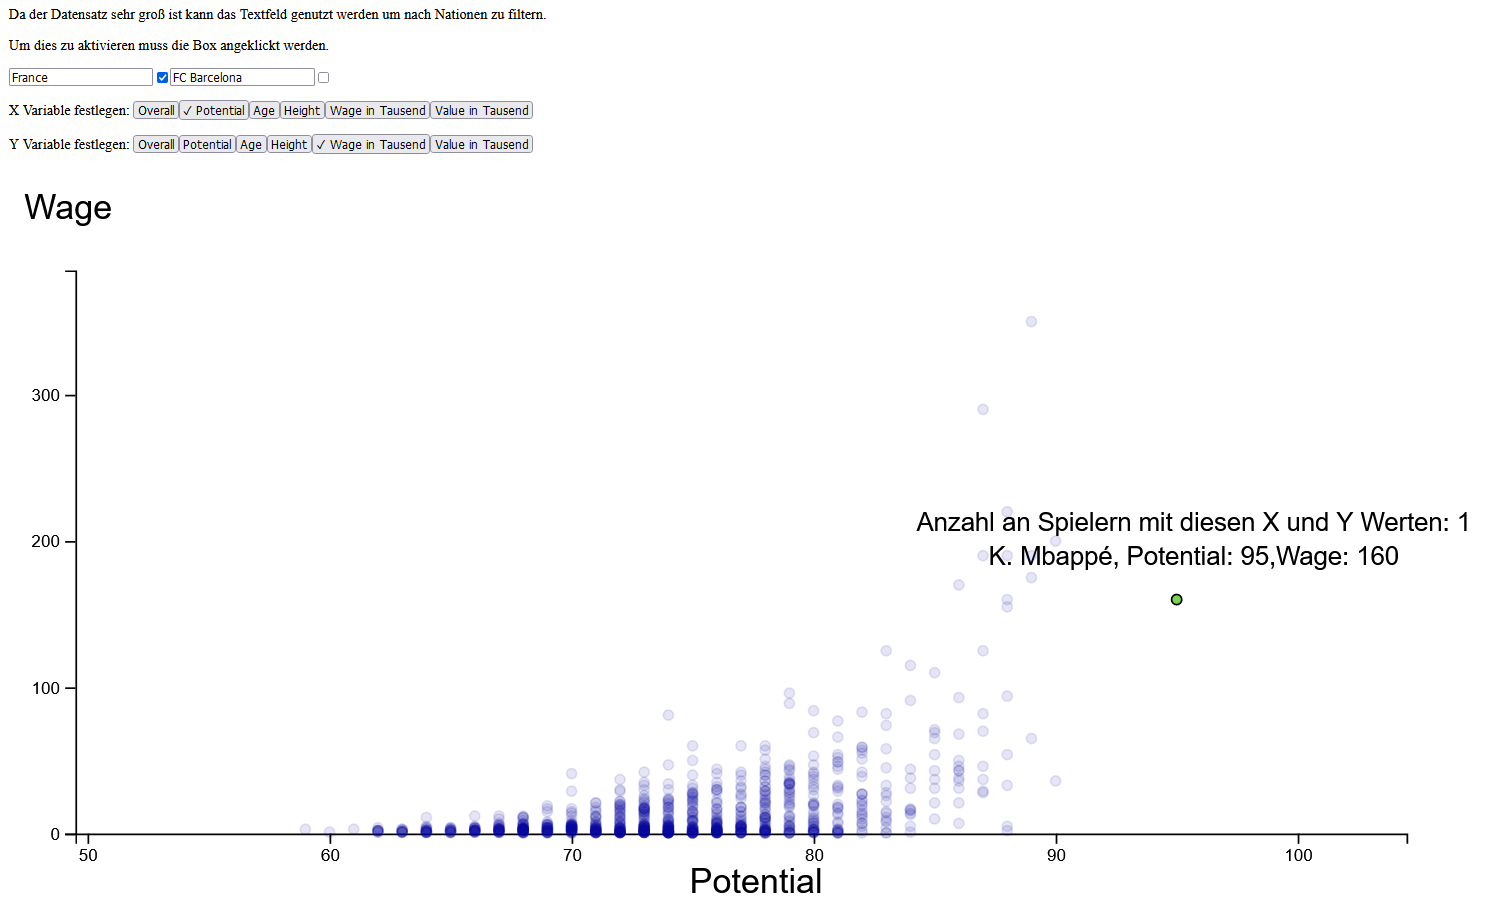
\includegraphics[scale=0.5]{grafiken/Scatterplot5}
\caption{Darstellung des Scatterplots und dessen \textit{on:hover} Funktionalität\\ Quelle: eigene Darstellung}
\label{SP5}
\end{figure}
Beispielhaft soll der Nutzen dieser Visualisierung anhand eines Spielers des Karrieremodus von FIFA 21 dargestellt werden.
Dieser Nutzer möchte für sein Team im Karrieremodus einen neuen Spieler finden. Dieser soll ein höchstmögliches Potential haben. Trotzdem soll das Gehalt des Fussballers bezahlbar sein. Weiterhin soll der Spieler Franzose sein. Aus diesem Grund vergleicht der Nutzer die Attribute \textit{Potential} und \textit{Wage} mit dem zusätzlichen Nationalitätenfilter \textit{France}. Dabei ist zu erkennen, dass mit steigendem Rating ab einem bestimmten Punkt das Gehalt exponential ansteigt. Ein Spieler, der zwar bereits ein sehr hohes Gehalt aufweist, für sein \textit{Potential} von 95 aber trotzdem vergleichsweise günstig ist, ist Kylian Mbappé. Dieser Spieler ist ein Ausreißer aus dem generellen Trend der exponentiell steigenden \textit{Wages} im Vergleich zum \textit{Potential}. Eine günstigere Option wäre in diesem Fall beispielsweise Dayot Upamecano, dessen Potential liegt zwar nur bei 90 das Gehalt allerdings auch nur bei 36000€. Dem Nutzer der Anwendung stehen so mehrere Optionen offen. Das Abweichen dieser Fussballer von Trends in den Daten wird erst durch diese Visualisierung offensichtlich.

\subsection{Anwendung Visualisierung Zwei}
In der Visualisierung der Parallelen Koordinaten werden in Abbildungen \ref{PK5} und \ref{PK51} die Attribute \textit{Defending, Physical, Pace} und \textit{Passing} mit einander verglichen.

\begin{figure}[h!]
\centering
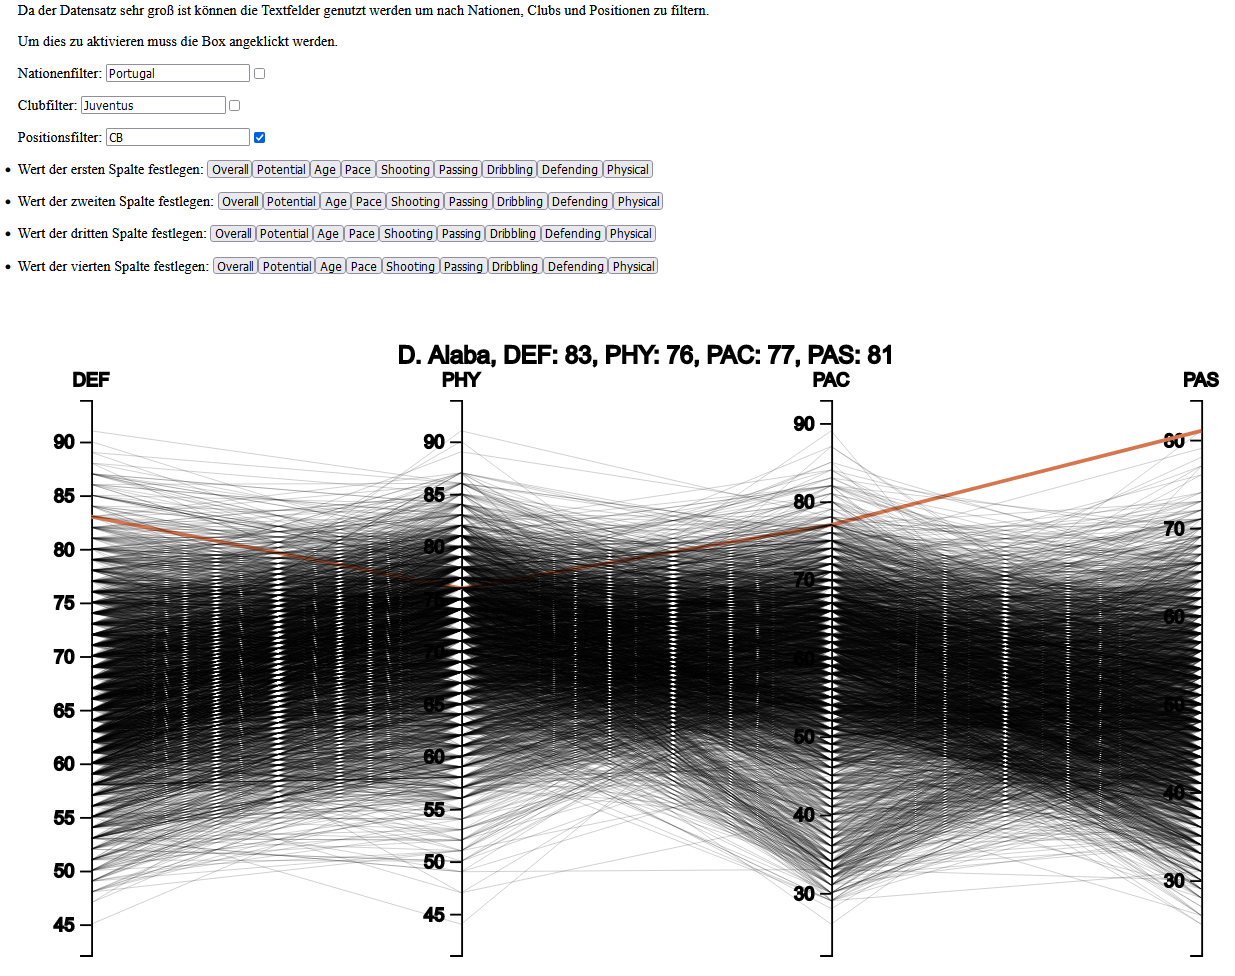
\includegraphics[scale=0.6]{grafiken/ParalleleKoordinaten5}
\caption{Darstellung der Parallelen Koordinaten inklusive \textit{on:hover} Funktionalität\\ Quelle: eigene Darstellung}
\label{PK5}
\end{figure}

\begin{figure}[h!]
\centering
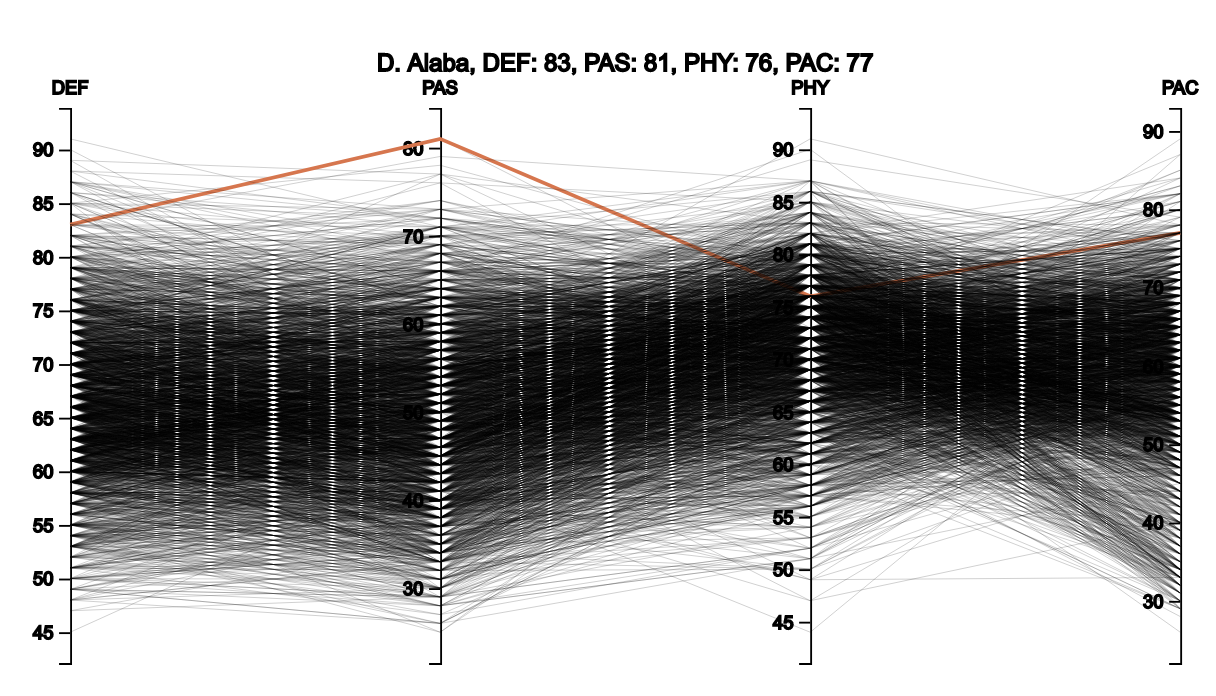
\includegraphics[scale=0.4]{grafiken/ParalleleKoordinaten51}
\caption{Abbildung 3 mit nach Links verschobenem\textit{Passing}\\ Quelle: eigene Darstellung}
\label{PK51}
\end{figure}

Beispielhaft soll der Nutzen dieser Visualisierung anhand der Anforderungen eines Spielers des FUT Modus von FIFA 21 dargestellt werden.
Dieser Anwender möchte sein Ultimate Team um einen Innenverteidiger (\textit{Centerback: CB}) erweitern. Neben den für einen Innenverteidiger typischerweise relevanten Attributen interessiert diesen Spieler auch die Passgenauigkeit des Innenverteidigers. Deswegen wählt er für den Vergleich die Attribute \textit{Defending, Physical, Pace} und \textit{Passing} aus. Generell ist bei Innenverteidigern in dieser Darstellung zu erkennen, dass die Passgenauigkeit im Vergleich zur Geschwindigkeit eher abfallend ist. Wird Abbildung \ref{PK51} betrachtet in der Passen um zwei Positionen in der Darstellung nach Links verschoben worden ist, ist  zu sehen, dass David Alaba entgegen des Trends - Passen ist im Vergleich zu Verteidigen und Physis eher geringer - einen höheren Passwert aufweist. Da die anderen Werte im Vergleich zu anderen Innenverteidigern trotzdessen hoch liegen bietet sich die Auswahl dieses Innenverteidigers für den Beispielnutzer an.

\subsection{Anwendung Visualisierung Drei}
In der Visualisierung der Baumdarstellung wird die Hierarchie von Bundesligavereinen inklusive Spielern der Position Rechtsverteidiger (Rightback: RB) gezeigt.
\begin{figure}[h!]
\centering
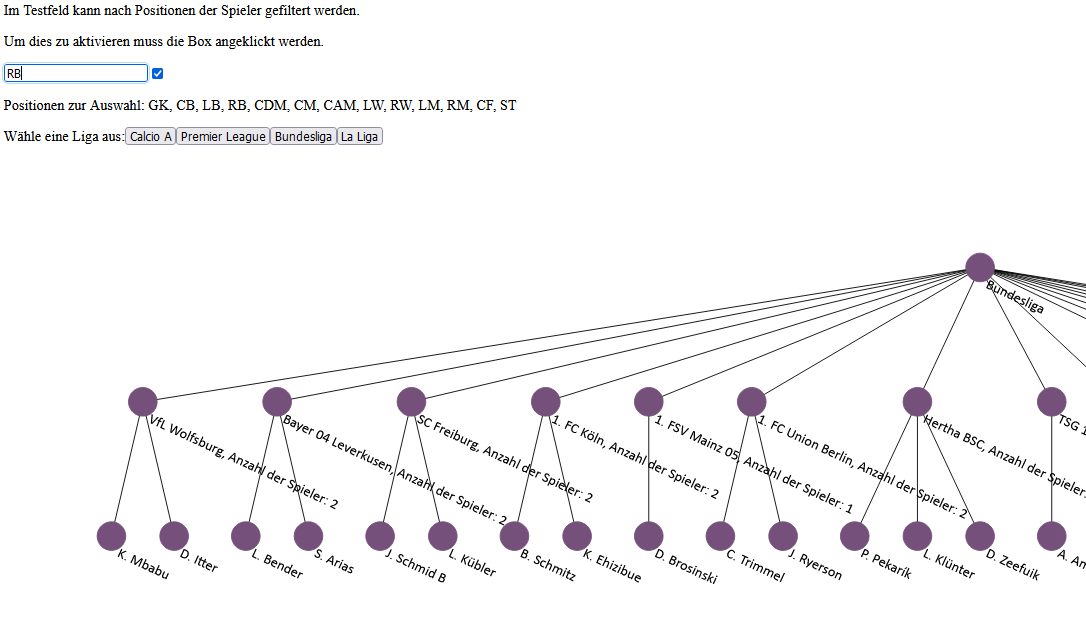
\includegraphics[scale=0.6]{grafiken/Baumdiagramm5}
\caption{Darstellung des Baumdiagramms\\ Quelle: eigene Darstellung}
\label{BD5}
\end{figure}

Beispielhaft wird diese wieder aus Sicht eines Spielers des FUT Modus betrachtet. In diesem Modus existiert ein Chemiesystem\cite{heib_fifa_2021}. Nach diesem System spielen nur Spieler gleicher Nation oder gleicher Liga gut miteinander. Weiterhin spielen Spieler gleicher Vereine besser zusammen. Ein Spieler ist dabei sich ein Team aus Spielern der Bundesliga zu bauen. Dabei fehlt allerdings ein Rechtsverteidiger. Um sich einen Überblick über die Rechtsverteidiger der Bundesliga zu verschaffen nutzt er die Funktionalität des Baumdiagramms. Dadurch werden ihm alle vorhandenen Bundesliga Rechtsverteidiger angezeigt. Ist es ihm wichtig, dass der Spieler für einen spezifischen Verein spielt so kann auch dies mit Hilfe dieser Visualisierungstechnik erkannt werden. Da die Menge der Kindelemente in dieser Anforderung keine Rolle spielt bietet sich Verwendung der expliziten Baumdarstellung im Vergleich zu den anderen, in Kapitel 3 diskutierten Techniken zur Darstellung hierarchischer Strukturen, an.



\section{Verwandte Arbeiten}

Da es sich bei den verwendeten Daten um die eines Videospiels handelt, existieren wenige wissenschaftliche Visualisierungen zu diesen. Allerdings existieren bereits einige nicht wissenschaftliche Visualisierungen, die hier kurz erwähnt werden sollen.
Zum einen ist dies die \textit{FIFA Data Visualization}\cite{ roshan_fifa_nodate} eine Visualisierung des FIFA 19 Datensatzes durch Roshan Sharma. In dieser Analyse der Daten werden verschiedene Werte des Datensatzes vor allem als Balken oder Kreisdiagramme dargestellt. Weiterhin werden Histogramme verwendet. Im Verlauf der Analyse werden auch, in dieser Veranstaltung konkreter behandelte Darstellungsformen wie bspw. der Scatterplot oder die Darstellung als Sternförmige Koordinaten, verwendet. Dabei liegt der Fokus auf der Darstellung von Mengenverteilungen verschiedener Attribute.

Eine nichtwissenschaftliche Visualisierung des, in dieser Arbeit verwendeten, FIFA 21 Datensatzes ist von Paramartha Sengupta durchgeführt worden. In \textit{FIFA 21: EDA and Visualization}\cite{sengupta_fifa_nodate} analysiert Sengupta  den Datensatz vor allem unter Einsatz von Scatterplots und Balkendiagrammen. Weiterhin werden Sterndiagramme verwendet um Attribute der Spieler zu vergleichen. Dabei beziehen sich die Analysen allerdings hauptsächlich auf aggregierte Daten und nicht auf spielerspezifische.
Allerdings werden mittels eines Scatterplots zwei Analysen durchgeführt, die so auch mit dem Scatterplot in dieser Arbeit durchgeführt werden können. In der ersten wird \textit{Age} von Spielern mit ihrem \textit{Overall} verglichen. In der zweiten wird das \textit{Age} der Spieler mit ihrem \textit{Potential} verglichen.\\

Um in der wissenschaftlichen Literatur vergleichbare Arbeiten zu finden muss sich vom Thema entfernt werden, zwar sind zum Videospiel FIFA keine wissenschaftlichen Artikel zu finden, jedoch lässt sich die hier durchgeführte Visualisierung mit der von Janetzko et. al.\cite{janetzko_enhancing_2016}, beruhend auf realen Fussballdaten, vergleichen.
In dieser Arbeit wird die Darstellungsform der Parallelen Koordinaten eingesetzt um Bewegungsdaten von Fussballern zu analysieren. Interessant ist dabei vor allem, dass die Darstellung aufgrund von Problemen der Erkennung von Clustern innerhalb der Achsen angepasst und um eine Farbkomponente erweitert worden ist. Weiterhin unterscheiden sich die Interaktionsmöglichkeiten im Vergleich zu denen dieser Arbeit deutlich. Es kann bspw. die Ober- und Untergrenze der Achsen verändert werden um so genauer in einzelne Cluster reinzoomen zu können. Weiterhin kann die Darstellung durch andere Visualisierungen überlagert werden.\\
Zwar lässt sich sagen, dass die Visualisierung gegenüber der aus dieser Arbeit einige Vorteile bietet. Es muss jedoch erwähnt werden, dass der Fokus bezüglich Zielgruppen der Arbeiten und damit auch den Anforderungen unterschiedlich liegt. In der vorgestellten Arbeit liegt der Fokus vor allem auf der Erkennung von Clustern innerhalb der Gesamtmenge der Daten. Im Gegensatz dazu liegt der Fokus dieser Arbeit darauf Ausreißer nach oben aus den vorhandenen Clustern zu identifizieren um so die bestmöglichen Spieler zu finden.
Bei einer möglichen Erweiterung dieser Arbeit wäre die Möglichkeit des manuellen Achsenskalierens trotzdem in Betracht zu ziehen.\\
Um die in der Einleitung gestellte Frage: \textit{Können die gegebenen Daten und Visualisierungen genutzt werden um auf reale Sportler rückschließen zu können?} beantworten zu können werden die Visualisierungen mit den Daten von Kalén et. al.\cite{kalen_are_2019} verglichen. In der Diskussion des Papers wird beschrieben, dass der Peak der Spielerleistung ungefähr im Alter von 31 Jahren erreicht wird. Diese Erkenntnis wird beim Betrachten des Scatterplots (X-Achse: \textit{Age}, Y-Achse: \textit{Overall}) ebenso erreicht, da in der Darstellung mit steigendem \textit{Age} ein steigendes \textit{Overall} zu erkennen ist. Dieses stagniert dann um das Alter von 31 und fällt danach wieder leicht ab. Somit lässt sich die Vermutung anstellen, dass die Daten auch Sportwissenschaftlern behilflich sein können. Trotzdem sind diese aufgrund ihrer Subjektivität mit Vorsicht zu betrachten. Lägen Realdaten vor, würden sich die Visualisierungen hingegen definitiv zur deren Darstellung eignen.    
%Führen sie eine kurze Literatursuche in der wissenschaftlichen Literatur zu Informationsvisualisierung und Visual Analytics nach ähnlichen Anwendungen durch. Diskutieren sie mindestens zwei Artikel. Stellen sie Gemeinsamkeiten und Unterschiede dar.
%\textbf{Zwei Artikel mit ähnlichen Zielen diskutieren}
\section{Zusammenfassung und Ausblick}
%Fassen sie die Beiträge ihre Visualisierungsanwendung zusammen. Wo bietet sie für die Personen der Zielgruppe einen echten Mehrwert.
Die Visualisierungen haben es ermöglicht aus einem unübersichtlichen Datensatz mit über 16000 Zeilen Informationen herauszufiltern und anschaulich darzustellen.
Anwendern ist es nach kurzer Einarbeitung möglich die Interaktionsmöglichkeiten der Visualisierungen selbst zu bedienen und auf neue Erkenntnisse zu stoßen. Dabei kann dies sowohl zum Sammeln von Informationen über einzelne Spieler, als auch zur Analyse größerer Trends getan werden. Besonders die Darstellungsform der Parallelen Koordinaten bietet im Vergleich zur Analyse der Daten als Liste einen echten Mehrwert, da Anwendern nicht nur die Werte der einzelnen Spieler angezeigt werden sondern durch die Pfade aller Spieler ein Maßstab für die Einschätzung der Werte einzelner Fussballer geschaffen wird. Zusammenfassend sind vor allem die Möglichkeit die Daten selbst filtern zu können,selbst Attribute der Achsen festzulegen sowie die \textit{on:hover} Funktionalität die großen Vorteile, die von den Visualisierungen geboten werden.\\
Mit Blick auf mögliche Verbesserungen der Visualisierungen fällt beim Scatterplot zum einen ein statt die Menge an gleichen Daten durch Opazität von einander zu unterscheiden dies mit Hilfe einer Farbskala zu tun. Ein weiterer Punkt der verbessert werden kann ist der Fakt, dass bei Überlagerung der Daten immer nur der Name eines Spielers angezeigt wird. Das Anzeigen einer Liste der Fussballer, die die gleichen Werte haben wäre da eine Verbesserungsmöglichkeit.\\
Die Parallelen Koordinaten könnten wie bereits in Kapitel 6 erwähnt um die Möglichkeit des manuellen Skalierens der Achsen erweitert werden um so das hereinzoomen in Cluster zu ermöglichen.\\
Im Fall des Baumdiagramms wäre es denkbar dieses um eine Funktion zu erweitern in der mehr Attribute der Spieler präsentiert werden. So könnten Anwender mehr nutzen aus dieser Visualisierung ziehen.\\ 
Abschließend ist zu sagen, dass trotz der Verbesserungsmöglichkeiten bereits durch die vorhandenen Visualisierungen ein echter Mehrwert gegenüber den Rohdaten an sich entsteht.



%\textbf{Beiträge der Anwendung, welcher Mehrwert für Zielgruppe entsteht, mögliche Erweiterungen(Visualisierungen oder Daten)}
%Was wären mögliche sinnvolle Erweiterungen, entweder auf der Ebene der Visualisierungen und/oder auf der Datenebene?

\newpage

\pagenumbering{Roman}
\setcounter{page}{4}
\addcontentsline{toc}{section}{Anhang: Git-Historie}
\section*{Anhang: Git-Historie}
Das die Commits von zwei verschiedenen Accounts stammen ist zu entschuldigen. Die Anmeldung in der GIT GUI von Windows ist unabsichtlich mit einem anderen Account vorgenommen worden und erst später bemerkt worden.

\begin{verbatim}
* ba194f5 (HEAD -> master, origin/master) (Writing Chapter 2, 2021-09-09)
* a32805e (Changes to html testsite, 2021-09-09)
* fcfa8fa (Updates to Scatterplot, 2021-09-08)
* 9f41152 (Added additional filterfunctionality to parallelCoordinates, 2021-09-08)
* 130d43d (Updated Readme.md, 2021-09-08)
* bcb2233 (changes to spData.csv reagrding encoding, 2021-09-08)
* 14007ce (Added filter functionality to parallel Coordinates, 2021-09-08)
* b373216 (deleted unused datasets, 2021-09-08)
* 75f726f (started writing chapter preprocessing, 2021-09-08)
* a2207bf (Renaming of elm files and Creation of elm files with smaller csv files, 2021-09-08)
* a2e9801 (fixed error in index.html, 2021-09-08)
* da0991c (Included new html file for parallel COordinates, 2021-09-08)
* 9f20f40 (Updated RDataPreprocessing file, 2021-09-08)
* c72d4a2 (Updated spData and spData2000 with value and wage, 2021-09-08)
* e46740a (test changes in spData.csv, 2021-09-08)
* 956bf26 (test update spDate, 2021-09-08)
* 379c0de (updated spData again, 2021-09-08)
* 477c43a (Updated spData.csv with wage and value data, 2021-09-08)
* 3c200e1 (Updated Baumdata.csv with Premier League Data, 2021-09-07)
* 3af31ee (Updated Baum csv data with serie a players, 2021-09-07)
* 1e66fcd (Development of Filterfunction for Players Positions in Treediagram, 2021-09-07)
* 1cfd18f (Updated Baumdata.csv, 2021-09-07)
* f5adf5f (reworking of 1.1, 2021-09-07)
* 1bd9293 (Creation of Tree.html, 2021-09-07)
* b04c990 (Created index.html for github pages, 2021-09-07)
* ebfba7f (Updated bibtex file, 2021-09-07)
* c6240a4 (First try of preprocessing parallel coordinates data, 2021-09-06)
* 43ba73b (Added highlighting and Player info on hover, 2021-09-06)
* 447a93e (changed additional errors in baumData.csv reagrding laLiga players, 2021-09-06)
* 30992b9 (fixed errors in LaLiga club names, 2021-09-06)
* 3a8659a (Updated Baumdata.csv with laliga clubs, 2021-09-06)
* 7a98e59 (Started writing preprocessing file in R, 2021-09-06)
* d4b3df2 (Changed error in Baumdata regarding multiple club names, 2021-09-06)
* c825fef (Created test csv Data for Baumdiagram, 2021-09-06)
* 79150e1 (Implementation of Filter function in the Scatterplot as well as changes to the selections, 2021-09-06)
* d3bc365 (-Created Fifa 21 Scatterplot Data, reduced to 2000 Players, 2021-09-05)
* 605e204 (Added preliminary Scatterplot Data from Fifa 21, 2021-09-05)
* cce366d (-Reorganization and inclusion of placeholder images, 2021-09-05)
* a6328bf (Added full csv of fifa 21 data to gitignore, 2021-09-05)
* abbce42 (started writing chapter 2.2, 2021-09-05)
* 1bcf321 (-Reorganized git 2 deleting additional, unused files, 2021-09-05)
* 0017063 (-Reorganized git, 2021-09-05)
* e5ebc82 (Updated Readme.me, 2021-09-05)
* 93b8a97 (-Started writing Chapter 2.1, 2021-09-05)
* 4477dba (Started writing chapter 1.3, 2021-09-05)
* 7be9390 (Started writing Chapter Zielgruppen, 2021-09-04)
* 2386040 (Reduced size of csv for testing purposes, 2021-08-22)
* 5d98177 (Added Nationality to CSV, 2021-08-22)
* a395085 (Added smaller CSV tree file, 2021-08-15)
* 4fa41ce (New Test CSV File for ElmTreeMap, 2021-08-15)
* 5952879 (Added .json file and Excercise tree visualization code to start implementing tree visualization, 2021-08-14)
* 1295900 (-Changed name of tex and pdf file and added new folder AbgabeOrdnerLatex, 2021-08-13)
* 5c1747d (-Changed gitignore to new Latex files, 2021-08-13)
* 9443014 (Kapitel 2 Daten Version 0.1, 2021-08-12)
* f673cd6 (-Grundlagen des Projektberichts, 2021-08-12)
* cd852b2 (TXT statt csv, 2021-08-12)
* 9c07724 (-Added smaller CSV with 1000 lines, 2021-08-12)
* a441b52 (-csv, 2021-08-12)
* 2f7fbe0 (-csv, 2021-08-12)
* 8ac06b8 (-minor fixes csv, 2021-08-12)
* cc9cede (Prefiltering of Data, 2021-08-12)
* eb68618 (Testing error with height, 2021-08-12)
* 95935c0 (Testing Height in Metres instead of CM, 2021-08-12)
* ef3a227 (Rounded Height, 2021-08-12)
* cb4c956 (Reduced CSV file, 2021-08-12)
* f0e6cae (Added Interactivity to parallel Coordinates, 2021-08-11)
* 9ee66e1 (Added Parallele Koordinaten Grundfunktionalität, 2021-08-11)
* eb4f173 (-Added Git Folder structure, 2021-08-11)
* 7d09347 (Added changeablity to the data, 2021-08-10)
* 07422d2 (Extended number of encodeable variables for the Scatterplot, 2021-08-06)
* a6fd816 (-Added possibility to change variables, 2021-08-03)
* f0f68ea (-Updated PointName -Started writing Paper, 2021-08-03)
* adfd7a6 (-First working Scatterplot, 2021-08-03)
* c4f4b5f (-Scatterplot first tries, 2021-08-03)
* f9af25c (-Commiting new files, 2021-07-30)
* 4618601 (Upload pdf, 2021-07-07)
* d267f3d (-deleted Latex files, 2021-07-07)
*   65fd4fd (Merge branch 'master' of https://github.com/Blauekuh/Visualisierung_FIFA19.git, 2021-07-07)
|\
| * 68629b2 (Update .gitignore, 2021-07-07)
* | 7aaf7f3 (Latex File created, 2021-07-07)
|/
* be4234d (-Added gitignore, 2021-07-05)
* 546ae0e (Upload CSV Dataset for Fifa 19, 2021-06-17)
* c640421 (Commit of first test elm file, 2021-06-16)
* fcdc3ad (origin/main, origin/Development) (Initial commit, 2021-06-16)
\end{verbatim}



\printbibliography

\end{document}

